\documentclass[12pt, a4paper]{article}
\usepackage[margin=1in, bottom=1.6in]{geometry}

% Include links
\usepackage{hyperref}

\usepackage{booktabs} % Table
\usepackage{caption}
\usepackage{enumitem} % Itemize letters

% Picture Packages
\usepackage{graphicx} % Include images
\usepackage{float}
\usepackage[dvipsnames]{xcolor} 
\usepackage{xcolor} % Highlight words with colour

\usepackage{adjustbox}

% Math packages
\usepackage{amsmath}  % Include the amsmath package
\usepackage{siunitx}
\usepackage{pgf} % Math Calculations
\usepgflibrary{fpu} % Process large numbers 
\pgfkeys{
    /pgf/fpu = true,
    /pgf/number format/.cd,
    precision=2,
    fixed,
    fixed zerofill,
    use comma,
    1000 sep={.}
}

% Add code into the report
\usepackage{listings}
\usepackage{color}

\definecolor{dkgreen}{rgb}{0,0.6,0}
\definecolor{gray}{rgb}{0.5,0.5,0.5}
\definecolor{mauve}{rgb}{0.58,0,0.82}

\lstset{frame=tb,
  language=Java,
  aboveskip=3mm,
  belowskip=3mm,
  showstringspaces=false,
  columns=flexible,
  basicstyle={\small\ttfamily},
  numbers=none,
  numberstyle=\tiny\color{gray},
  keywordstyle=\color{blue},
  commentstyle=\color{dkgreen},
  stringstyle=\color{mauve},
  breaklines=true,
  breakatwhitespace=true,
  tabsize=3
}

\begin{document}
\title{Truss Weight Optimization}
\author{George D.}
\maketitle{}

\section{PROBLEM STATEMENT}

(A problem taken from Mechanics of Materials, 4th edition, Craig, Taleff, John Wiley & Sons, 2020.) 

The pin-jointed planar truss shown in the figure below is to be made of two steel two-force members and support a single vertical load P = 15kN at joint B. For the steel truss members, the allowable stress in tension is $(\sigma_\text{T})_\text{allow}=150 \text{MPa}$, the allowable stress in compression is $(\sigma_\text{C})_\text{allow}=-80 \text{MPa}$, and the weight density is $77.2 \frac{\text{kN}}{\text{m}^3}$. You are to consider truss designs for which joint B can be located at any point along the vertical line that is 1m to the right of AC, with a $y_B$ varying from $y_B=0$ to $y_B = 2m$

\begin{figure}[H]
    \centering
    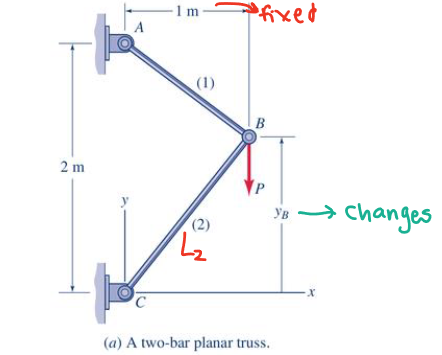
\includegraphics[width=0.5\linewidth]{problem.png}
    \caption{Two-Bar Planar Truss System, Labeled}
\end{figure}

\newpage
\section{EQUATIONS}

Equations and explanations to be added.

% \begin{equation}
%     \begin{aligned} 
%     \end{aligned}
% \end{equation}

\newpage
\section{RESULTS AND CALCULATIONS}

The following code was used to create this simulation:

\begin{lstlisting}
    import matplotlib.pyplot as plt
    import numpy as np

    g = 77.2 * 10**3
    P = 15 * 10**3
    s_tallow = 150 
    s_callow = -80
    x = P/2

    a = np.linspace(0, 2, 20)
    l_one = np.sqrt(1**2 + (2-a)**2)
    l_two = np.sqrt(1 + a**2)

    W = g * (x * ((l_one**2 / s_tallow) - (l_two**2 / s_callow)))

    # Index of the minimum value of W
    min_index = np.argmin(W)

    # Minimum W value and corresponding "a" value
    min_a = a[min_index]
    min_W = W[min_index]
    print(f"Minimum W: {min_W} at $y_B$ = {min_a}")

    # Index where a = 0
    a_0_index = np.where(a == 0)[0][0]
    W_0 = W[a_0_index]
    print(f"At a = 0, W = {W_0}")
    plt.scatter(0, W_0, color='blue', zorder=5, label=f'({0}, {W_0})')

    # graph of W vs "a" or (y_B)
    plt.plot(a, W, 'r', label="W vs $y_B$")

    # Minimum W on graph 
    plt.scatter(min_a, min_W, color='blue', zorder=5, label=f'Min W ({min_a:.2f}, {min_W:.2f})')
    plt.text((min_a*0.60), (min_W+0.125*10**7), f'({min_a:.2f}, {min_W:.2f})')

    # Title and Labels
    plt.xlabel('Position of Joint B ($y_B$)')
    plt.ylabel('Weight of Truss (W)')
    plt.title('Weight of Truss vs. Position of Joint B')

    plt.legend() # Legend

    plt.show()
\end{lstlisting}

From this code, the following graph was produced: 

\begin{figure}[H]
    \centering
    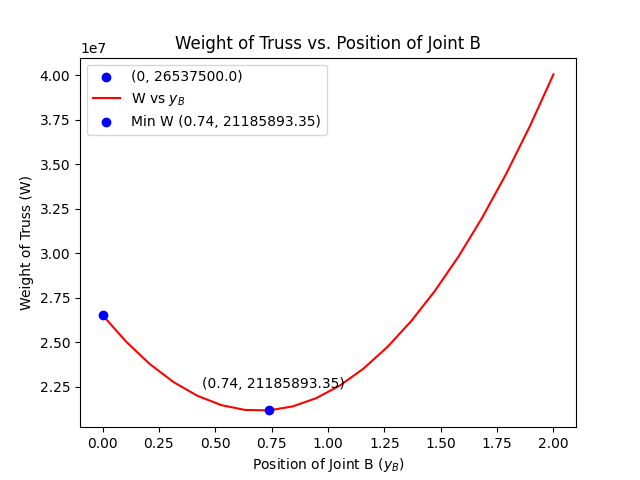
\includegraphics[width=0.8\linewidth]{graphresult.png}
    \caption{Weight of Truss vs. Position of Joint B y_B}
\end{figure}

Thus, the optimal weight of the truss is 21185893 N, or 21186 kN. 

% \section{DISCUSSIONS AND CONCLUSION}

% \textbf{Discussions go here.}

% \section{REFERENCES}

% [1] Toronto Metropolitan University. (n.d.). Computer Assignment. \\ 
% \indent Retrieved Month, #, 2023, from \url{https://} \\ \\ 

\end{document}